%%%%%%%%%%%%
%% Please rename this main.tex file and the output PDF to
%% [lastname_firstname_graduationyear]
%% before submission.
%%
%% This .tex file is for use with BibLaTeX. Please use
%% main-bibtex.tex instead if you prefer BibTeX.
%%%%%%%%%%%%

\documentclass[12pt]{caltech_thesis}
\usepackage[hyphens]{url}
\usepackage{lipsum}
\usepackage{graphicx}

\usepackage{todonotes}
\usepackage{physics}

%% Tentative: newtx for better-looking Times
\usepackage[utf8]{inputenc}
\usepackage[T1]{fontenc}
\usepackage{newtxtext,newtxmath}
% Must use biblatex to produce the Published Contents and Contributions, per-chapter bibliography (if desired), etc.
\usepackage[
    backend=biber,natbib,
    % IMPORTANT: load a style suitable for your discipline
    style=nature
]{biblatex}
\usepackage{nomencl}


\makenomenclature
%% This code creates the groups
% -----------------------------------------
\usepackage{etoolbox}
\renewcommand\nomgroup[1]{%
  \item[\bfseries
  \ifstrequal{#1}{M}{Molecular orbital basis}{%
  \ifstrequal{#1}{N}{Number sets}{%
  \ifstrequal{#1}{O}{Other symbols}{}}}%
]}
% -----------------------------------------

\usepackage{listings} % Required for insertion of code
\usepackage{xcolor} % Required for custom colors

% Define custom colors
\definecolor{codegreen}{rgb}{0,0.6,0}
\definecolor{codegray}{rgb}{0.5,0.5,0.5}
\definecolor{codepurple}{rgb}{0.58,0,0.82}
\definecolor{backcolour}{rgb}{0.95,0.95,0.92}

% Setup the style for code listings
\lstdefinestyle{mystyle}{
    backgroundcolor=\color{backcolour},   
    commentstyle=\color{codegreen},
    keywordstyle=\color{magenta},
    numberstyle=\tiny\color{codegray},
    stringstyle=\color{codepurple},
    basicstyle=\ttfamily\footnotesize,
    breakatwhitespace=false,         
    breaklines=true,                 
    captionpos=b,                    
    keepspaces=true,                 
    numbers=left,                    
    numbersep=5pt,                  
    showspaces=false,                
    showstringspaces=false,
    showtabs=false,                  
    tabsize=2
}

% Activate the style
\lstset{style=mystyle}
\usepackage{hyperref}

% Name of your .bib file(s)
\addbibresource{examples.bib}
\addbibresource{ownpubs.bib}

\begin{document}

% Do remember to remove the square bracket!
\title{$G_0W_0$ for Molecules}
\author{Patryk Kozlowski}

\degreeaward{Bachelor of Science in Chemistry}                 % Degree to be awarded
\university{California Institute of Technology}    % Institution name
\address{Pasadena, California}                     % Institution address
\unilogo{caltech.png}                                 % Institution logo
\copyyear{2024}  % Year (of graduation) on diploma
\defenddate{[Exact Date]}          % Date of defense

\orcid{0009-0000-6402-4261}

%% IMPORTANT: Select ONE of the rights statement below.
\rightsstatement{All rights reserved}
% \rightsstatement{All rights reserved except where otherwise noted}
% \rightsstatement{Some rights reserved. This thesis is distributed under a [name license, e.g., ``Creative Commons Attribution-NonCommercial-ShareAlike License'']}

%%  If you'd like to remove the Caltech logo from your title page, simply remove the "[logo]" text from the maketitle command
\maketitle[logo]
%\maketitle

\begin{acknowledgements} 	 
   [Add acknowledgements here. If you do not wish to add any to your thesis, you may simply add a blank titled Acknowledgements page.]
\end{acknowledgements}

\begin{abstract}
   [This abstract must provide a succinct and informative condensation of your work. Candidates are welcome to prepare a lengthier abstract for inclusion in the dissertation, and provide a shorter one in the CaltechTHESIS record.]
\end{abstract}

%% Uncomment the `iknowhattodo' option to dismiss the instruction in the PDF.


\tableofcontents
\listoffigures
\listoftables
\printnomenclature

\mainmatter

\chapter{Nomenclature}
This uses the restricted Hartree-Fock formalism, meaning that two electrons with opposite spin occupy each spatial orbital.\\\\
\begin{tabular}{p{0.65\textwidth} p{0.8\textwidth}}
Symbol & Description \\
\hline
\(i,j,k,l\) & Occupied orbital indices \\
\(a,b,c,d\) & Virtual orbital indices \\
\(p,q,r,s\) & General MO indices \\
\(\mu,\nu,\lambda,\sigma\) & AO indices \\
\((pq|rs) = \int \int \psi_p^*(\mathbf{r}_1)\psi_q(\mathbf{r}_1)\frac{1}{r_{12}}\psi_r^*(\mathbf{r}_2)\psi_s(\mathbf{r}_2)d\mathbf{r}_1d\mathbf{r}_2\) & Two-electron integrals \\
\((pq||rs) = (pq|rs) - (ps|rq)\) & Antisymmetrized two-electron integrals \\

\end{tabular}\\\\
All calculations have been done using the PySCF package.\autocite{sun_recent_2020} The code for this project can be found at \url{https://github.com/pkozlows/gw_senior_thesis/tree/master}.
\chapter{Motivation}
The formalism of many-body perturbation theory (MBPT) provides corrections to a mean-field description such as that given by Hartree-Fock or density functional theory (DFT). The former method does not treat electron correlation at all, and the latter one treats it in an average way. DFT is often used for systems of large size, as it is fairly accurate and computationally cheap. However, DFT's reliance on empirically based functionals in some cases gives rise to the notorious self-interaction error; because one is considering an electron in the average field of the electrons in the system, you can have an electron interacting with itself. In practice, this can potentially lead to a variety of issues, including the underestimation of surface stability (overestimation of surface energies) relevant in surface science studies. \autocite{schimka_accurate_2010} To remedy this problem, normally one would fall back onto the wave function-based MBPT methods, such as coupled cluster theory (CC) and Moller-Plesset perturbation theory to 2nd order (MP2). However, their computational scaling is steep for larger systems, such as periodic ones.\autocite{mcclain_gaussian-based_2017} Because of this issue, the perturbative methods often are not a better option than the field-standard DFT in predicting the properties of materials, as I have learned in a previous study.\autocite{kozlowski_elucidating_2021} Therefore, in the quantum chemistry community, there has been an interest in applying Green's function MBPT methods, with the $GW$ approximation, to such systems, which has shown to give accurate corrections to, for example, band gaps, on top of a prior (DFT) mean-field calculation, at a cheap computational cost.\autocite{noauthor_frontiers_nodate} This is the motivation for my study of the $G_0W_0$ method.
\newpage
Figure \ref{fig:water_homo} quantifies the potential of greens function methods, such as $G_0W_0$. As can be seen, $G_0W_0$ lowers the orbital energy and, thus, captures more of the electronic correlation, as desired.
\begin{figure}[h]
    \centering
    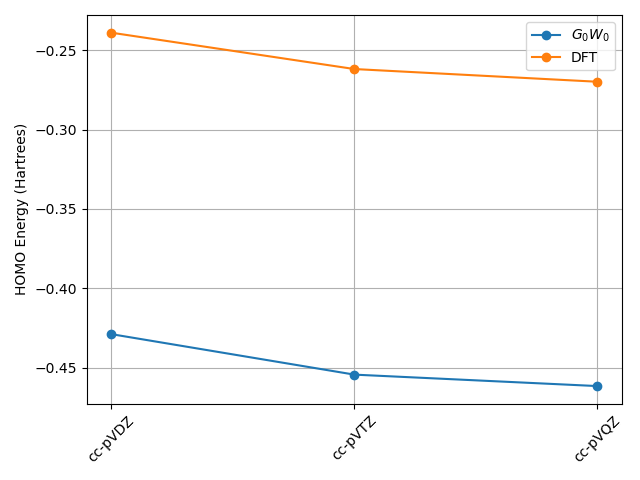
\includegraphics[width=\textwidth]{water_gw.png}
    \caption{Difference in the HOMO energy for the water molecule with different bases (cc-pVDZ, etc.) for $G_0W_0$, and DFT, both starting from the PBE functional}
    \label{fig:water_homo}
\end{figure}


\chapter{Theoretical Background}
We begin by writing out the Schrödinger equation for the $N$-electron system in a molecular field. 
\begin{equation}
    \hat{H}\Psi =E\Psi 
\end{equation}
with
\begin{equation}
\hat{H}=\sum_{i=1}^N\left(-\frac{1}{2} \nabla_i^2\right)-\sum_{i=1}^N \sum_{\alpha }\frac{Z_{\alpha }}{r_{i\alpha }}+\sum_{i<j}^N \frac{1}{r_{i j}}
\end{equation}
We note that we do not include the potential energy term associated with the nuclear-nuclear repulsion, as we are working in the Born-Oppenheimer approximation. This can be succinctly written as the sum of a kinetic energy term with a nuclear-electronic attraction term and an electron-electron repulsion term  
\begin{equation}
    \hat{H}= \hat{T}+ \hat{V}_{ne}+\hat{V}_{ee}
\end{equation}
The objective of many years of research in quantum chemistry has been solving for the $V_{ee}$ term. Now, I will introduce some of the mean field methods that have been classically used to tackle this problem at a cheap computational cost.
\section{Mean Field Methods}
\subsection{Hartree-Fock}
In the restricted Hartree-Fock formalism, the $V_{ee}$ is given by
\begin{equation}
    V_{ee} = \frac{1}{2} \sum_i^{\text {occ }} \sum_j^{\text {occ }} 2(ii|jj) - (ij|ji)
\end{equation}
The first term is the Coulomb term and the second term is an exchange term. We choose to make the following presentation in the restricted Hartree-Fock formalism, but considering spin here is important. In the unrestricted Hartree-Fock formalism, this would be given by
\begin{equation}
    V_{ee} = \frac{1}{2} \sum_{\underline{i}}^{\text{occ}} \sum_{\underline{j}}^{\text{occ}} \left( (\underline{i}\underline{i}|\underline{j}\underline{j}) - (\underline{i}\underline{j}|\underline{j}\underline{i}) \right)
\end{equation}
Where the underline denotes that these are spin orbitals; we have not performed the summation over all possible spins yet. The Hartree-Fock method fails to take into account the exchange term in the unrestricted case; the integral vanishes when the spins of $i$ and $j$ are different. Physically, this means that there is no energetic stabilization for two electrons with different spins to occupy the same spatial index, whereas there is one when the spins are parallel. This was what was meant earlier by the statement that Hartree-Fock does not treat electron correlation.\autocite{szabo_modern_2012}
\subsection{Density Functional Theory (DFT)}
The central quantity in DFT is the electron density, as represented by a density matrix. The method is fairly black box, and its intricate details will not be covered here (for further reading see \textcite{bruneval_assessment_2019}), but it is important to understand that it treats the electron correlation through an exchange-correlation functional, which in principle has an exact form, but in practice is approximated as semi-empirical, which leads to issues in accurately describing the electron correlation from an ab-initio perspective.\\\\
What is important to understand is that both of these mean field methods yield molecular orbital energies $\epsilon_{p}$ and coefficients $C_{\mu p}$, which we correct with MBPT methods.
\section{Many-body perturbation theory}
There are many different MBPT methods, but they all have the same purpose of recovering a portion of the electron correlation missed by these mean field methods. For example, Hartree-Fock is variational, meaning that its energy $E_{HF}$ will always be greater or equal to the true energy of the system $E_0$. For HF, we define the difference between these two quantities as the correlation energy
\begin{equation}
    E_{\text{corr}} \equiv E_0 - E_{HF}
\end{equation}
The other mean field method that is often used is DFT, but it is not variational, so there is not such a simple interpretation of $E_{\text{corr}}$ in this case, but the principle is similar. We will be focusing on recovering electron correlation with the $G_0W_0$ method, which is a Green's function-based MBPT method.



\chapter{$G_0W_0$ Procedure}
\section{Iterative equation}
The procedure that we used to compute quasiparticle energies, which are interpreted as effective molecular orbital energies, is given by 
\begin{equation}
    \delta_{pq}F_{pq}^{HF}[\gamma^{DFT}] + \Sigma^{corr}(\varepsilon_{p}^{QP}) = \varepsilon_{p}^{QP}.
\label{eq: Iterative equation}
\end{equation}
We explain the notation starting from left to right. The first term corresponds to taking the diagonal of the Hartree-Fock matrix $F_{pq}^{HF}$ evaluated at a given electron density $\gamma$. These electron densities are obtained from a previous mean-field calculation, either $\gamma_{DFT}$ or $\gamma_{HF}$. The one-electron reduced density matrix is used to express the electron density here. The second term evaluates $\Sigma^{corr}$ for the $\varepsilon_{p}^{QP}$ determined in the previous iteration. The right side of the equality gives the updated $\varepsilon_{p}^{QP}$.\\\\ Equation \ref{eq: Iterative equation} is iterated until self-consistency. We start with an initial guess for $\varepsilon_{p}^{QP}$, which is given by the mean-field orbital energy $\epsilon_p$. This is used in the first iteration to solve for the right-hand side $\varepsilon_{p}^{QP}$ of Equation \ref{eq: Iterative equation}. In the next iteration, we use the previously obtained $\varepsilon_{p}^{QP}$ to determine $\Sigma^{corr}$. This process is repeated until we reach a convergence threshold for $\varepsilon_{p}^{QP}$.
\subsection{The Fock Matrix}
In the basis of atomic orbitals, the HF Fock matrix is
\begin{equation}
F_{\mu\nu}^{HF} = h_{\mu\nu} + \sum_{\lambda\sigma}P_{\lambda\sigma}(\mu\nu|\lambda\sigma) - \frac{1}{2}\sum_{\lambda\sigma}P_{\lambda\sigma}(\mu\lambda|\nu\sigma)
\label{eq: Fock matrix}
\end{equation}
where $h_{\mu\nu}$ is the one-electron part of the Hamiltonian, $P_{\lambda\sigma}$ is the one-electron reduced density matrix, and $(\mu\nu|\lambda\sigma)$ is a two-electron integral. \autocite{szabo_modern_2012} A useful identity for $P_{\lambda\sigma}$ in terms of the MO coefficients from the mean-field calculation is: 
\begin{equation}
P_{\mu\nu} = 2\sum_{i=1}^{N/2}C_{\mu i}C_{\nu i}^{*}
\end{equation}
We note that the sum runs only over the $N/2$ occupied \emph{spatial} orbitals. Equation \ref{eq: Fock matrix} is the form for the HF Fock matrix, and not the DFT Fock matrix. In the canonical HF MO basis, $F_{\mu\nu}^{HF}$ merely has the HF MO energies placed on the diagonal. We transform the Fock matrix into the MO basis with
\begin{equation}
   F_{pq} = \sum_{\mu} \sum_{\nu} C_{\mu p}^{*}F_{\mu\nu}C_{\nu q}
\end{equation}
where $C$ is the matrix of MO coefficients.
\subsection{Correlation-Self Energy}
$\Sigma^{corr}$ is the second term in Equation \ref{eq: Iterative equation} and is the central quantity in the $GW$ method. It is formed from the inputted Green's function $G$ and the screened Coulomb potential $W$ and recovers a portion of the $E_{corr}$ mentioned earlier. $\Sigma^{corr}$ is dynamic, as opposed to the previous Fock term that was discussed, as is updated with a new $\varepsilon_{p}^{QP}$ in each iteration. In the case of the $G_0W_0$ approximation, we use the common approximation, considering only the diagonal element of $\Sigma^{corr}$ corresponding to the orbital with index $p$. This function is evaluated at the $\varepsilon_{p}^{QP}$ just obtained in the previous iteration. To summarize, we are actually interested in $\Sigma_{pp}^{corr}(\varepsilon_{p}^{QP})$. We will go into greater detail about the form of $\Sigma^{corr}$ in the next chapter.
\subsection{Updated $\varepsilon_{p}^{QP}$}
This is the right side, or the solution, of Equation \ref{eq: Iterative equation}.
\newpage
\subsection{Graphical solution}
We are able to check Equation \ref{eq: Iterative equation} in the HF case by plotting $\Sigma^{corr}$ as a function of the input frequency, which takes on  the possible values for $\varepsilon_{p}^{QP}$. Since $F_{pq}^{HF}$ is diagonal in the canonical HF MO basis, Equation \ref{eq: Iterative equation} can be reformulated as
\begin{equation}
    \epsilon _{p}^{HF} + \Sigma_{pp}^{corr}(\omega) = \omega  \rightarrow \Sigma_{pp}^{corr}(\omega) = \omega  - \epsilon _{p}^{HF}
\end{equation}
Essentially, the line at $\omega - \epsilon_{p}^{HF}$ should, and does, intersect with $\Sigma^{corr}$ at the same $\varepsilon_{p}^{QP}$ that we get from our iterative procedure, namely at the $\omega = -12.18 eV$.
 This is a useful check to see if the self-energy, which we will derive in the next chapter, is being computed correctly.

\begin{figure}[h]
    \centering
    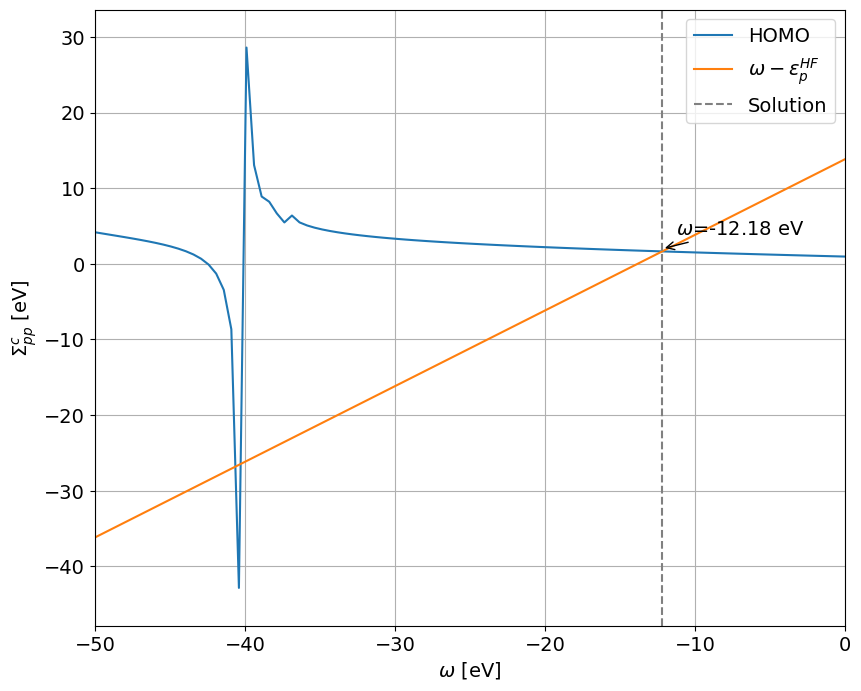
\includegraphics[width=\textwidth]{correlation_energies.png}
\end{figure}
Also, at around $\omega$ = -40 eV, one can observe a pole structure. This would pose problems for the convergence of my iterative procedure Equation \ref{eq: Iterative equation} if the $\varepsilon_{p}^{QP}$ that I was looking for was close to this $\omega $ value, but luckily $-12.18 eV$ is far enough away from this pole at $-40 eV$.


\section{Correlation Self-Energy}
\begin{equation}
    \Sigma_{pp}^{\text{corr}}(\omega) = \sum_{\mu }^{\text{RPA}}\left(\sum_{i}^{\text{occupied}} \frac{\textbf{V}_{pi}^{\mu }\textbf{V}_{ip}^{\mu }}{\omega -(\epsilon _{i}-\Omega  _{\mu })}+ \sum_{a}^{\text{virtual}} \frac{\textbf{V}_{pa}^{\mu }\textbf{V}_{ap}^{\mu }}{\omega -(\epsilon _{a}+\Omega  _{\mu })}\right)
\end{equation}
This is the working equation for the diagonal of the correlation self-energy for a given MO. The $\textbf{V}^{\mu}$ and $\Omega_{\mu}$ are the excitation vectors and energies, respectively, from a previous RPA calculation. $\omega$ is my input frequency and the $\epsilon$ are the orbital energies from my previous mean-field calculation.



\section{Random Phase Approximation}
The RPA is a linear response theory that is used to compute the excitation energies and vectors. The working matrix equation is given by \autocite{dreuw_single-reference_2005}:
\begin{equation}
\begin{bmatrix}
A & B \\
-B & -A
\end{bmatrix}
\begin{bmatrix}
X \\
Y
\end{bmatrix}
= \omega
\begin{bmatrix}
1 & 0 \\
0 & -1
\end{bmatrix}
\begin{bmatrix}
X \\
Y
\end{bmatrix}
\end{equation}
where $A$ is
\begin{equation}
    \textbf{A}_{ia,jb} = \delta _{ij}\delta _{ab}(\varepsilon _{a}- \varepsilon _{i}) + 2(ia||jb)
\label{eq: A matrix RPA}
\end{equation}
and $B$ is
\begin{equation}
    \textbf{B}_{ia,jb} = 2(ia||jb)
\label{eq: B matrix RPA}
\end{equation}

We can work to simplify this eigenvalue problem. Since we know that the negative and positive eigenvalues for the RPA are the same in magnitude, we can simplify the matrix equation to:
\begin{equation}
\begin{bmatrix}
A & B \\
-B & -A
\end{bmatrix}
\begin{bmatrix}
X \\
Y
\end{bmatrix}
= \omega
\begin{bmatrix}
X \\
Y
\end{bmatrix}
\end{equation}
This suggests breaking down the problem into a set of linear equations:
\begin{align}
    AX + BY &= \omega X\\
    -BX-AY &= \omega Y
\end{align}
which can be simplified by the addition:
\begin{equation}
    (A-B)(X-Y)= \omega (X+Y)
\end{equation}
which means:
\begin{equation}
    (X+Y) = \omega^{-1}(A-B)(X-Y)
\label{eqn:addition}
\end{equation}
Doing the subtraction instead gives:
\begin{equation}
    (A+B)(X+Y)= \omega (X-Y)
\label{eqn:for_subtraction}
\end{equation}
Similarly, we can isolate:
\begin{equation}
    (X-Y) = \omega^{-1}(A+B)(X+Y)
\label{eqn:subtraction}
\end{equation}
Substituting in for $X+Y$ from \ref{eqn:addition} into equation \ref{eqn:for_subtraction}:
\begin{equation}
    \omega^{-1}(A+B)(A-B)(X-Y) = \omega (X-Y)
\end{equation}
Multiplication by $\omega$ gives:
\begin{equation}
    (A+B)(A-B)(X-Y) = \omega^2 (X-Y)
\end{equation}
Now, we plug the defintion in \ref{eqn:subtraction} for the $(X-Y)$ terms:
\begin{equation}
    (A+B)(A-B)\omega^{-1}(A+B)(X+Y) = \omega^2 \omega^{-1}(A+B)(X+Y)
\end{equation}
Multiplication through by $\omega$ gives and $(A+B)^{-1}$ gives:
\begin{equation}
    (A-B)(A+B)(X+Y) = \omega^{2} (X+Y)
\end{equation}
At this point we want to define $T=(A-B)^{-\frac{1}{2}}(X+Y)$, so that we can write:
\begin{equation}
    (A-B)(A+B)(A-B)^{\frac{1}{2}}T = \omega^{2} (A-B)^{\frac{1}{2}}T
\end{equation}
Dividing through by $(A-B)^{\frac{1}{2}}$ gives:
\begin{equation}
    (A-B)^{\frac{1}{2}}(A+B)(A-B)^{\frac{1}{2}}T = \omega^{2} T
\end{equation}


The excitation vectors $\textbf{V}^{\mu}$ are taken by considering a contraction of two tensors. First, we consider the sum of $\textbf{X}$ and $\textbf{Y}$ at the same excitation energy $\mu$: $\textbf{Z}_{i,a,\mu} = \textbf{X}_{i,a,\mu} + \textbf{Y}_{i,a,\mu}$. Then we contract this with the two-electron integrals:
\begin{equation}
    \textbf{W}_{p,q,i,a} = \sqrt{2} \sum_{p,q,i,a} (pq|ia)
\end{equation}
This factor of $\sqrt{2}$ comes from the spin integration of the restricted Hartree-Fock formalism.
We defined a combined occupied-virtual index $\nu$, so: $\textbf{Z}_{i,a,\mu} \rightarrow \textbf{Z}_{\nu, \mu}$ and $\textbf{W}_{p,q,i,a}\rightarrow \textbf{W}_{p,q,\nu}$.\\

% Inline Python code in the document
And then we form the excitation vector from:
\begin{equation}
    \textbf{V}_{pq}^{\mu} = \sum_{\nu} \textbf{W}_{p,q,\nu}\textbf{Z}_{\nu, \mu}
\end{equation}

\subsection{Tamm-Dancoff Approximation}
In this method, we neglect the $\textbf{B}$ matrix of the RPA equation. So the eigenvalue equation becomes
\begin{equation}
    \textbf{A}\textbf{X} = \omega \textbf{X}
\end{equation}
where we still have:
\begin{equation}
    \textbf{A}_{ia,jb} = \delta _{ij}\delta _{ab}(\varepsilon _{a}- \varepsilon _{i}) + 2(ia||jb)
\label{eq: A matrix TDA}
\end{equation}
And then we follow the same procedure as in the RPA to get $\textbf{V}_{pq}^{\mu}$, where now we have $\textbf{Z}_{\nu, \mu} = \textbf{X}_{\nu, \mu}$.
\subsection{Direct approximation}
Everywhere in the code, we consider the direct approximation, which just means that all instances of anti-symmetrized two-electron integrals are replaced by their non-symmetrized counterparts. In Equation \ref{eq: A matrix RPA}, Equation \ref{eq: B matrix RPA}, and Equation \ref{eq: A matrix TDA}, $(ia||jb) \rightarrow (ia|jb)$. In the former case it was called the \emph{direct} Random Phase Approximation (dRPA) and in the latter case it was called the \emph{direct} Tamm-Dancoff Approximation (dTDA).
\chapter{Linearized $G_0W_0$ Density Matrix}
\subsection{Implementation}
These are the working equations for the linearized $G_0W_0$ Density Matrix that I will derive later. \autocite{bruneval_assessment_2019} First, we consider the fully occupied block:
\begin{equation}
\gamma_{i j}^{G W}=2\delta_{i j}-2\sum_{a \mu} \frac{\textbf{V}_{i a}^\mu \textbf{V}_{ja}^\mu}{\left(\epsilon_{i}-\epsilon_{a}-\Omega_{\mu}\right)\left(\epsilon_{j}-\epsilon_{a}-\Omega_{\mu}\right)}
\end{equation}
where the $\Omega_{\mu}$ are the excitation energies and the $\textbf{V}^{\mu}$ are the excitation vectors. The sum runs over all virtual orbitals and excitation energies. The $\epsilon$ are the orbital energies from the prior mean-field calculation. Next, we have the virtual-virtual block:
\begin{equation}
\gamma_{a b}^{G W}=-2\sum_{i \mu } \frac{\textbf{V}_{a i}^{\mu} \textbf{V}_{b i}^{\mu}}{\left(\epsilon_{i}-\epsilon_{a}-\Omega_{\mu}\right)\left(\epsilon_{i}-\epsilon_{b}-\Omega_{\mu}\right)}
\end{equation}
Finally, we have the mixed block:
\begin{equation}
    \gamma_{i b}^{G W}=\frac{2}{\epsilon_{i}-\epsilon_{b}}\left[ \sum_{a \mu} \frac{\textbf{V}_{i a}^{\mu} \textbf{V}_{b a}^{\mu}}{\epsilon_{i}-\epsilon_{a}-\Omega_{\mu}} - \sum_{j \mu} \frac{\textbf{V}_{i j}^{\mu} \textbf{V}_{bj}^{\mu}}{\epsilon_{j}-\epsilon_{b}-\Omega_{\mu}} \right]
\end{equation}
This all contributes to the form of the density matrix as:
\begin{equation}
    2\begin{pmatrix}
        \gamma _{i j}^{G W} & \gamma _{i b}^{G W} \\
        \gamma _{bi}^{G W } & \gamma _{a b}^{G W}
    \end{pmatrix}
\end{equation}
Where $\gamma _{bi}^{G W }$ is simply the transpose of $\gamma _{ib}^{\text{GW}}$, since all elements of this matrix are real. Therefore, this density matrix is Hermitian. The factor of 2 comes from the fact that we sum over both spins in the restricted Hartree-Fock formalism.
\newpage
\subsection{Plotting natural occupations}
The natural occupations is found by diagonalizing the density matrix. They are interpreted as being the number of electrons in a given orbital.\autocite{szabo_modern_2012} Here we considered the one-electron density matrix from multiple methods: We considered restricted Hartree-Fock, which contains no correlation, and Full Configuration Interaction (FCI), which contains the exact correlation. As can be seen in Figure \ref{fig:h2_dissociation}, our implementation of the Linearized $G_0W_0$ Density Matrix in the direct Random Phase Approximation (dRPA) and direct Tamm-Dancoff Approximation (dTDA) gives a portion of this correlation. It is interesting to see that the dTDA contains more correlation than the dRPA, as the former is a subset of the latter, and so the latter should recover more correlation.
\begin{figure}[h]
    \centering
    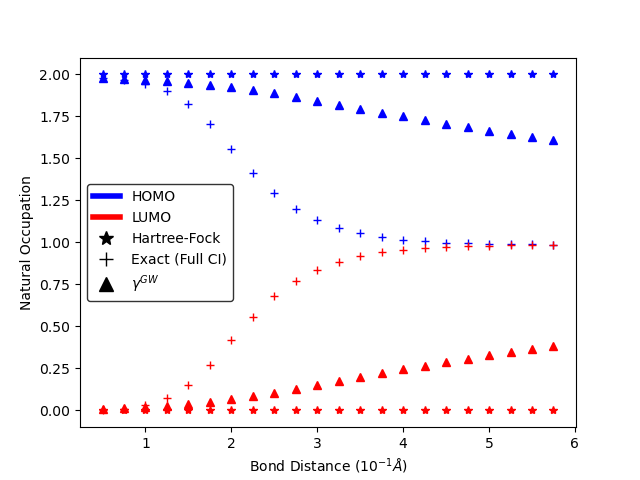
\includegraphics[width=\textwidth]{h2_occupations.png}
\caption{Natural occupations of the HOMO (State 1) and LUMO (State 2) of $H_2$ along the dissociation coordinate}
\label{fig:h2_dissociation}
\end{figure}
When $H_2$ is at its equilibrium distance at a low bond distance, we see in Figure \ref{fig:h2_dissociation} that the HOMO is fully occupied with 2 electrons, while the LUMO is unoccupied. This situation is represented by the simple MO diagram in Figure \ref{fig:h2_mo_diagram}. As the molecule dissociates, the occupations for the restricted Hartree-Fock method do not change at all, while FCI, containing the exact correlation, gives the expected result of the HOMO and LUMO both having occupations of 1 electron. The dRPA and dTDA fall somewhere in between these two extremes.
\begin{figure}[h]
    \centering
    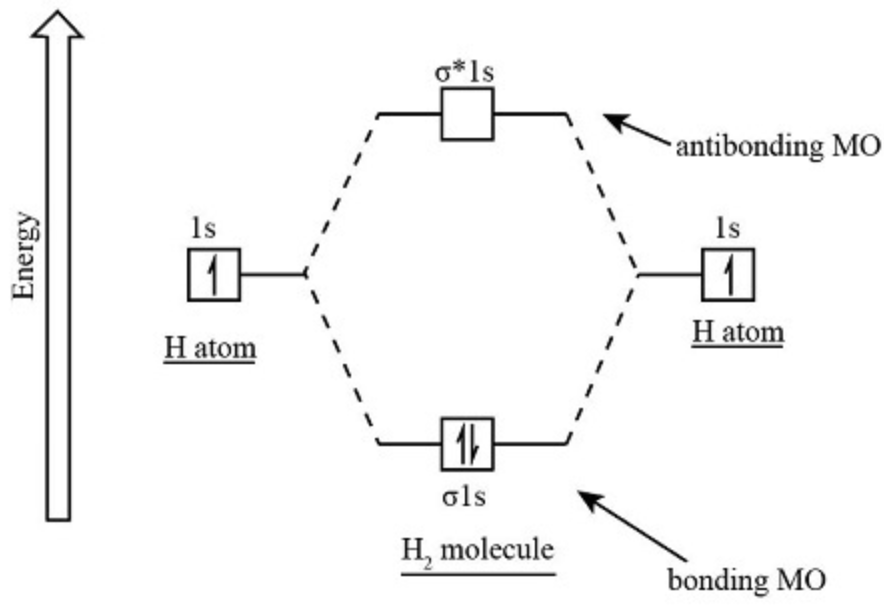
\includegraphics[width=\textwidth]{h2_mo.png}
\caption{MO diagram of $H_2$ at the equilibrium bond distance. Notice that the HOMO is fully occupied with 2 electrons, while the LUMO is unoccupied. Figure from \textcite{bruneval_assessment_2019}}
\label{fig:h2_mo_diagram}
\end{figure}


\chapter{This is the Sixth Chapter}
\chapter{This is the Seventh Chapter}
\chapter{This is the Eighth Chapter}

\printbibliography[heading=bibintoc]

\appendix

\chapter{Derivation of the linearized $G_0W_0$ density matrix}
We have the equation for the density matrix:
\begin{equation}
\begin{aligned}
\gamma^\sigma\left(\mathbf{r}_1, \mathbf{r}_2\right)= & \gamma_0^\sigma\left(\mathbf{r}_1, \mathbf{r}_2\right) -\frac{\mathrm{i}}{2 \pi} \int \mathrm{d} \mathbf{r}_3 \mathrm{~d} \mathbf{r}_4 \mathrm{~d} \omega \mathrm{e}^{\mathrm{i \omega \eta}} G_0^\sigma\left(\mathbf{r}_1, \mathbf{r}_3, \omega\right) \Sigma_c^\sigma\left(\mathbf{r}_3, \mathbf{r}_4, \omega\right) G_0^\sigma\left(\mathbf{r}_4, \mathbf{r}_2, \omega\right)
\label{eqn:init_dm}
\end{aligned}
\end{equation}
In order to simplify the integral, Let us consider
\begin{equation}
I = \int \mathrm{d} \mathbf{r}_3 \mathrm{~d} \mathbf{r}_4  G_0^\sigma\left(\mathbf{r}_1, \mathbf{r}_3\right) \Sigma_c^\sigma\left(\mathbf{r}_3, \mathbf{r}_4\right) G_0^\sigma\left(\mathbf{r}_4, \mathbf{r}_2\right)
\end{equation}
The noninteracting Green's function is defined as:
\begin{equation}
G_0\left(\mathbf{r}_1, \mathbf{r}_2, \right) = \sum_{pq} \phi_p^*(\mathbf{r}_1) G_{p q} \phi_q(\mathbf{r}_2)
\end{equation}
and likewise for the self-energy:
\begin{equation}
\Sigma_c\left(\mathbf{r}_1, \mathbf{r}_2, \right) = \sum_{pq} \phi_p^*(\mathbf{r}_1) \Sigma_{c pq} \phi_q(\mathbf{r}_2)
\end{equation}
where $G_{p q}$ and $\Sigma_{p q}$ are the matrix elements of the noninteracting Green's function and the self-energy, respectively. We can rewrite the integral as:
\begin{equation}
I = \sum_{pq} \sum_{rs} \sum_{tu} \int \mathrm{d} \mathbf{r}_3 \mathrm{~d} \mathbf{r}_4 \phi_p^*(\mathbf{r}_1) G_{p q} \phi_q(\mathbf{r}_3) \phi_r^*(\mathbf{r}_3) \Sigma_{r s} \phi_s(\mathbf{r}_4) \phi_t^*(\mathbf{r}_4) G_{t u} \phi_u(\mathbf{r}_2)
\end{equation}
We can simplify this expression by using the orthonormality of the basis functions:
\begin{equation}
I = \sum_{pq} \sum_{r} \sum_{t} \phi_p^*(\mathbf{r}_1) G_{p r} \phi_r(\mathbf{r}) \phi_r^*(\mathbf{r}) \Sigma_{r t} \phi_t(\mathbf{r}^\prime) \phi_t^*(\mathbf{r}^\prime) G_{t q} \phi_q(\mathbf{r}_2)
\end{equation}
We use this and then also rewrite equation \ref{eqn:init_dm} in terms of the matrix elements of the density matrix using the following definition:
\begin{equation}
D_{p q \sigma}=\left\langle p \sigma\left|\gamma^\sigma\right| q \sigma\right\rangle
\end{equation}
By the derivation above, we can rewrite equation \ref{eqn:init_dm} as:
\begin{equation}
    D_{p q \sigma}=\bra{p\sigma } \gamma _0^\sigma \ket{q\sigma } -\frac{\mathrm{i }}{2 \pi} \sum_{r} \sum_{t} \int_{-\infty }^{\infty } \mathrm{d} \omega \mathrm{e}^{\mathrm{i \omega \eta}} \bra{p\sigma } G_0^\sigma (\omega) \ket{r\sigma } \bra{r\sigma } \Sigma_c^\sigma (\omega) \ket{t\sigma } \bra{t\sigma } G_0^\sigma (\omega) \ket{q\sigma }
\label{eqn:mo_dm}
\end{equation}
Next, we plug in the following definitions into equation \ref{eqn:mo_dm}:
\begin{equation}
G_{0 p q}^\sigma=\sum_i \frac{\delta_{p q} \delta_{p i}}{\omega-\epsilon_{i \sigma}-\mathrm{i} \eta}+\sum_a \frac{\delta_{p q} \delta_{p a}}{\omega-\epsilon_{a \sigma}+\mathrm{i} \eta}
\end{equation}
and
\begin{equation}
\begin{aligned}
\Sigma_{c p q}^\sigma(\omega)= & \sum_{i s} \frac{w_{p i \sigma}^s w_{q i \sigma}^s}{\omega-\epsilon_{i \sigma}+\Omega_s-\mathrm{i} \eta} +\sum_{a s} \frac{w_{p a \sigma}^s w_{q a \sigma}^s}{\omega-\epsilon_{a \sigma}-\Omega_s+\mathrm{i} \eta}
\end{aligned}
\end{equation}
to get:
\begin{equation}
\begin{aligned}
D_{p q \sigma}= & \bra{p\sigma } \gamma _0^\sigma \ket{q\sigma } -\frac{\mathrm{i }}{2 \pi} \sum_{r} \sum_{t} \int_{-\infty }^{\infty } \mathrm{d} \omega \mathrm{e}^{\mathrm{i \omega \eta}} \left( \sum_i \frac{\delta_{p r} \delta_{p i}}{\omega-\epsilon_{i \sigma}-\mathrm{i} \eta}+\sum_a \frac{\delta_{p r} \delta_{p a}}{\omega-\epsilon_{a \sigma}+\mathrm{i} \eta} \right)\\
& \left( \sum_{k s} \frac{w_{r k \sigma}^s w_{t k \sigma}^s}{\omega-\epsilon_{k \sigma}+\Omega_s-\mathrm{i} \eta} +\sum_{c s} \frac{w_{r c \sigma}^s w_{t c \sigma}^s}{\omega-\epsilon_{c \sigma}-\Omega_s+\mathrm{i} \eta} \right) \left( \sum_j \frac{\delta_{t q} \delta_{t j}}{\omega-\epsilon_{j \sigma}-\mathrm{i} \eta}+\sum_b \frac{\delta_{t q} \delta_{t b}}{\omega-\epsilon_{b \sigma}+\mathrm{i} \eta} \right)
\end{aligned}
\end{equation}
Let us just distribute the integral, which technically spawns 8 terms. Also note that the delta functions will get rid of the sums over r and t:
\begin{equation}
\begin{aligned}
I = \int_{-\infty }^{\infty }\mathrm{d} \omega \mathrm{e}^{\mathrm{i \omega \eta}} 
& \left( \sum_{ijks} \left( \frac{w_{i k \sigma}^s w_{j k \sigma}^s}{(\omega-\epsilon_{k \sigma}+\Omega_s-\mathrm{i} \eta)(\omega-\epsilon_{i \sigma}-\mathrm{i} \eta)(\omega-\epsilon_{j \sigma}-\mathrm{i} \eta)} \right) \right.\\
& \left. + \sum_{ibks} \left( \frac{w_{i k \sigma}^s w_{b k \sigma}^s}{(\omega-\epsilon_{k \sigma}+\Omega_s-\mathrm{i} \eta)(\omega-\epsilon_{i \sigma}-\mathrm{i} \eta)(\omega-\epsilon_{b \sigma}+\mathrm{i} \eta)} \right) \right.\\
& \left. + \sum_{ijcs} \left( \frac{w_{i c \sigma}^s w_{j c \sigma}^s}{(\omega-\epsilon_{c \sigma}-\Omega_s+\mathrm{i} \eta)(\omega-\epsilon_{i \sigma}-\mathrm{i} \eta)(\omega-\epsilon_{j \sigma}-\mathrm{i} \eta)} \right) \right.\\
& \left. + \sum_{ibcs} \left( \frac{w_{i c \sigma}^s w_{b c \sigma}^s}{(\omega-\epsilon_{c \sigma}-\Omega_s+\mathrm{i} \eta)(\omega-\epsilon_{i \sigma}-\mathrm{i} \eta)(\omega-\epsilon_{b \sigma}+\mathrm{i} \eta)} \right) \right. \\
& \left. + \sum_{ajks} \left( \frac{w_{a k \sigma}^s w_{j k \sigma}^s}{(\omega-\epsilon_{k \sigma}+\Omega_s-\mathrm{i} \eta)(\omega-\epsilon_{a \sigma}+\mathrm{i} \eta)(\omega-\epsilon_{j \sigma}-\mathrm{i} \eta)} \right) \right.\\
& \left. + \sum_{abks} \left( \frac{w_{a k \sigma}^s w_{b k \sigma}^s}{(\omega-\epsilon_{k \sigma}+\Omega_s-\mathrm{i} \eta)(\omega-\epsilon_{a \sigma}+\mathrm{i} \eta)(\omega-\epsilon_{b \sigma}+\mathrm{i} \eta)} \right) \right.\\
& \left. + \sum_{ajcs} \left( \frac{w_{a c \sigma}^s w_{j c \sigma}^s}{(\omega-\epsilon_{c \sigma}-\Omega_s+\mathrm{i} \eta)(\omega-\epsilon_{a \sigma}+\mathrm{i} \eta)(\omega-\epsilon_{j \sigma}-\mathrm{i} \eta)} \right) \right.\\
& \left. + \sum_{abcs} \left( \frac{w_{a c \sigma}^s w_{b c \sigma}^s}{(\omega-\epsilon_{c \sigma}-\Omega_s+\mathrm{i} \eta)(\omega-\epsilon_{a \sigma}+\mathrm{i} \eta)(\omega-\epsilon_{b \sigma}+\mathrm{i} \eta)} \right) \right)
\label{eqn:expanded_integral}
\end{aligned}
\end{equation}
At this point, we note the following relation between integrals $\oint_{D_{\pm}} f(z) = \int_{-R}^R f(z) + \int_{{C_R}_{\pm}} f(z)$. $D_{\pm}$ is a semicircular domain in either half of the complex plane, ${C_R}_{\pm}$ is the semicircle in the upper or lower part of the complex plane, and $R$ is the radius of the semicircle. We are able to take $R\rightarrow \infty$ and since $f(z)=e^{i\omega \eta}g(z)$, where $g(z)$ is analytic on $D$ except for a finite number of poles, the integral over the semicircle will vanish by Jordan's lemma, leaving us with $\int_{-R=-\infty}^{R=\infty} f(z)= \oint_{D_{\pm}} f(z)$. 
\section{Fully occupied block}
The contribution over the fully occupied block of the density matrix will be given by the following two terms in equation \ref{eqn:expanded_integral}:
\begin{equation}
\begin{aligned}
I_{ij} =& \sum_{ks} w_{i k \sigma}^s w_{j k \sigma}^s \oint_{D+} \mathrm{d} \omega \mathrm{e}^{\mathrm{i \omega \eta}} \frac{1}{(\omega-\epsilon_{k \sigma}+\Omega_s-\mathrm{i} \eta)(\omega-\epsilon_{i \sigma}-\mathrm{i} \eta)(\omega-\epsilon_{j \sigma}-\mathrm{i} \eta)}\\
& + \sum_{cs} w_{i c \sigma}^s w_{j c \sigma}^s \oint_{D+} \mathrm{d} \omega \mathrm{e}^{\mathrm{i \omega \eta}} \frac{1}{(\omega-\epsilon_{c \sigma}-\Omega_s+\mathrm{i} \eta)(\omega-\epsilon_{i \sigma}-\mathrm{i} \eta)(\omega-\epsilon_{j \sigma}-\mathrm{i} \eta)}
\end{aligned}
\end{equation}
Due to the contour $D_+$ chosen for this case, we have poles for the first term at $\omega_{11} = \epsilon _{k\sigma } - \Omega _s + \mathrm{i} \eta$, $\omega_{12} = \epsilon _{i\sigma } + \mathrm{i} \eta$, and $\omega_{13} = \epsilon _{j\sigma } + \mathrm{i} \eta$. For such simple poles, the Cauchy residue theorem simplifies to:
\begin{equation}
\operatorname{Res}_{\omega =\omega _0} f(\omega )= \phi^{}\left(\omega _0\right)
\label{eqn:cauchy_residue}
\end{equation}
where $\phi_{\omega _0}(\omega ) = (\omega - \omega_0) f(\omega )$. For the first of these integrals in the occupied block, we have:
\begin{equation}
f_1(\omega) = \frac{e^{i\omega \eta }}{(\omega-\epsilon_{k \sigma}+\Omega_s-\mathrm{i} \eta)(\omega-\epsilon_{i \sigma}-\mathrm{i} \eta)(\omega-\epsilon_{j \sigma}-\mathrm{i} \eta)}
\end{equation}
% Plugging in $\omega_{11} = \epsilon _{k\sigma } - \Omega _s + \mathrm{i} \eta$, we get:
% \begin{equation}
% \phi_{\omega_{11}}(\omega) = (\omega - \epsilon_{k \sigma} + \Omega_s - \mathrm{i} \eta) f_1(\omega) = \frac{e^{i\omega \eta }}{(\omega-\epsilon_{i \sigma}-\mathrm{i} \eta)(\omega-\epsilon_{j \sigma}-\mathrm{i} \eta)}
% \end{equation}
So at the first pole, in the limit $\eta \to 0$, we get:
\begin{equation}
\phi_{\omega_{11}}(\epsilon_{k \sigma} - \Omega_s + \mathrm{i} \eta) = \frac{1}{(\epsilon_{k \sigma} - \Omega_s -\epsilon_{i \sigma})(\epsilon_{k \sigma} - \Omega_s -\epsilon_{j \sigma})}
\end{equation}
For the other poles, the procedure is similar:
\begin{equation}
\phi_{\omega_{12}}(\epsilon_{i \sigma} + \mathrm{i} \eta) = \frac{1}{(\epsilon_{i \sigma} -\epsilon_{k \sigma}+\Omega_s)(\epsilon_{i \sigma} -\epsilon_{j \sigma})}
\end{equation}
\begin{equation}
\phi_{\omega_{13}}(\epsilon_{j \sigma} + \mathrm{i} \eta) = \frac{1}{(\epsilon_{j \sigma} -\epsilon_{k \sigma}+\Omega_s)(\epsilon_{j \sigma} -\epsilon_{i \sigma})}
\end{equation}
We move on to the second integral in the occupied block. It only has two poles in the fully occupied contour: $\omega_{21} = \epsilon _{i\sigma } + \mathrm{i} \eta$ and $\omega_{22} = \epsilon _{j\sigma } + \mathrm{i} \eta$. We have $f_2(\omega)$ as:
\begin{equation}
f_2(\omega) = \frac{e^{i\omega \eta }}{(\omega-\epsilon_{c \sigma}-\Omega_s+\mathrm{i} \eta)(\omega-\epsilon_{i \sigma}-\mathrm{i} \eta)(\omega-\epsilon_{j \sigma}-\mathrm{i} \eta)}
\end{equation}
So $\phi_{\omega_{21}}(\omega _{21})$ is:
\begin{equation}
\phi_{\omega_{21}}(\epsilon_{i \sigma} + \mathrm{i} \eta) = \frac{1}{(\epsilon_{i \sigma} -\epsilon_{c \sigma}-\Omega_s)(\epsilon_{i \sigma} -\epsilon_{j \sigma})}
\end{equation}
Now we consider the second pole at $\omega_{22} = \epsilon _{j\sigma } + \mathrm{i} \eta$
\begin{equation}
\phi_{\omega_{22}}(\epsilon_{j \sigma} + \mathrm{i} \eta) = \frac{1}{(\epsilon_{j \sigma} -\epsilon_{c \sigma}-\Omega_s)(\epsilon_{j \sigma} -\epsilon_{i \sigma})}
\end{equation}
We summarize the results in a table \ref{tab:poles_residues_occupied}:\\
\begin{table}[h]
\centering
\caption{Summary of Poles and their Residues}
\begin{tabular}{|c|c|c|}
\hline
Pole Notation & Position $\omega_0$ & Residue $\phi_{\omega_0}(\omega_0)$ \\
\hline
\multicolumn{3}{|c|}{Series $\omega_1$} \\
\hline
$\omega_{11}$ & $\epsilon_{k \sigma} - \Omega_s + \mathrm{i} \eta$ & $\frac{1}{(\epsilon_{k \sigma} - \Omega_s -\epsilon_{i \sigma})(\epsilon_{k \sigma} - \Omega_s -\epsilon_{j \sigma})}$ \\
$\omega_{12}$ & $\epsilon_{i \sigma} + \mathrm{i} \eta$ & $\frac{1}{(\epsilon_{i \sigma} -\epsilon_{k \sigma}+\Omega_s)(\epsilon_{i \sigma} -\epsilon_{j \sigma})}$ \\
$\omega_{13}$ & $\epsilon_{j \sigma} + \mathrm{i} \eta$ & $\frac{1}{(\epsilon_{j \sigma} -\epsilon_{k \sigma}+\Omega_s)(\epsilon_{j \sigma} -\epsilon_{i \sigma})}$ \\
\hline
\multicolumn{3}{|c|}{Series $\omega_2$} \\
\hline
$\omega_{21}$ & $\epsilon_{i \sigma} + \mathrm{i} \eta$ & $\frac{1}{(\epsilon_{i \sigma} -\epsilon_{c \sigma}-\Omega_s)(\epsilon_{i \sigma} -\epsilon_{j \sigma})}$ \\
$\omega_{22}$ & $\epsilon_{j \sigma} + \mathrm{i} \eta$ & $\frac{1}{(\epsilon_{j \sigma} -\epsilon_{c \sigma}-\Omega_s)(\epsilon_{j \sigma} -\epsilon_{i \sigma})}$ \\
\hline
\label{tab:poles_residues_occupied}
\end{tabular}
\end{table}
Adding the two terms together, we get:
\begin{equation}
\begin{aligned}
I_{ij} = 2\pi i \Bigg( & \sum_{ks} w_{i k \sigma}^s w_{j k \sigma}^s \left( \frac{1}{(\epsilon_{k \sigma} - \Omega_s - \epsilon_{i \sigma})(\epsilon_{k \sigma} - \Omega_s - \epsilon_{j \sigma})} + \frac{1}{(\epsilon_{i \sigma} - \epsilon_{k \sigma} + \Omega_s)(\epsilon_{i \sigma} - \epsilon_{j \sigma})} \right. \\
& \left. + \frac{1}{(\epsilon_{j \sigma} - \epsilon_{k \sigma} + \Omega_s)(\epsilon_{j \sigma} - \epsilon_{i \sigma})} \right) \\
& + \sum_{cs} w_{i c \sigma}^s w_{j c \sigma}^s \left( \frac{1}{(\epsilon_{i \sigma} - \epsilon_{c \sigma} - \Omega_s)(\epsilon_{i \sigma} - \epsilon_{j \sigma})} + \frac{1}{(\epsilon_{j \sigma} - \epsilon_{c \sigma} - \Omega_s)(\epsilon_{j \sigma} - \epsilon_{i \sigma})} \right) \Bigg)
\end{aligned}
\end{equation}
Getting a common denominator for all of the terms means that the first term simplifies to 0, and the second term gives:
\begin{equation}
I_{ij} = -2\pi i \sum_{cs}\frac{w_{i c \sigma}^s w_{j c \sigma}^s}{(\Omega_s + \epsilon_{c \sigma} - \epsilon_{i \sigma})(\Omega_s + \epsilon_{c \sigma} - \epsilon_{j \sigma})}
\end{equation}
So, the expression for $D_{ij}$ is:
\begin{equation}
D_{ij} = \bra{i\sigma } \gamma _0^\sigma \ket{j\sigma } + \frac{2\pi i^2}{2\pi} \sum_{cs}\frac{w_{ic} w_{jc}}{(\Omega_s + \epsilon_{c \sigma} - \epsilon_{i \sigma})(\Omega_s + \epsilon_{c \sigma} - \epsilon_{j \sigma})}
\end{equation}
The first term is the matrix element of the noninteracting part of the density matrix, so this just simplifies to $\delta _{ij}$ and then we relabel the virtual index $c\rightarrow a$:
\begin{equation}
D_{ij} = \delta _{ij} - \sum_{as}\frac{w_{ia} w_{ja}}{(\Omega_s + \epsilon_{a \sigma} - \epsilon_{i \sigma})(\Omega_s + \epsilon_{a \sigma} - \epsilon_{j \sigma})}
\end{equation}
\section{Fully Virtual Block}
For the fully virtual block, we need to consider third to last and last terms of the integral in equation \ref{eqn:expanded_integral}:
\begin{equation}
\begin{aligned}
I_{ab} =& \sum_{ks} w_{a k \sigma}^s w_{b k \sigma}^s \int \mathrm{d} \omega \mathrm{e}^{\mathrm{i \omega \eta}} \frac{1}{(\omega-\epsilon_{k \sigma}+\Omega_s-\mathrm{i} \eta)(\omega-\epsilon_{a \sigma}+\mathrm{i} \eta)(\omega-\epsilon_{b \sigma}+\mathrm{i} \eta)}\\
& + \sum_{cs} w_{a c \sigma}^s w_{b c \sigma}^s \int \mathrm{d} \omega \mathrm{e}^{\mathrm{i \omega \eta}} \frac{1}{(\omega-\epsilon_{c \sigma}-\Omega_s+\mathrm{i} \eta)(\omega-\epsilon_{a \sigma}+\mathrm{i} \eta)(\omega-\epsilon_{b \sigma}+\mathrm{i} \eta)}
\end{aligned}
\end{equation}
Due to the contour $D_-$ chosen for this case, we have poles for the first term at just $\omega_{11} = \epsilon _{a \sigma } - \mathrm{i} \eta$ and $\omega_{12} = \epsilon _{b \sigma } - \mathrm{i} \eta$. Using the Cauchy residue theorem from equation \ref{eqn:cauchy_residue}:
\begin{equation}
f_1(\omega) = \frac{e^{i\omega \eta }}{(\omega-\epsilon_{k \sigma}+\Omega_s-\mathrm{i} \eta)(\omega-\epsilon_{a \sigma}+\mathrm{i} \eta)(\omega-\epsilon_{b \sigma}+\mathrm{i} \eta)}
\end{equation}
Plugging in $\omega_{11} = \epsilon _{a \sigma } - \mathrm{i} \eta$, we get:
% \begin{equation}
% \phi_{\omega_{11}}(\omega) = (\omega - \epsilon_{a \sigma} + \mathrm{i} \eta) f_1(\omega) = \frac{e^{i\omega \eta }}{(\omega-\epsilon_{k \sigma}+\Omega_s-\mathrm{i} \eta)(\omega-\epsilon_{b \sigma}+\mathrm{i} \eta)}
% \end{equation}
% Evaluating this at the pole, we get:
% \begin{equation}
% \phi_{\omega_{11}}(\epsilon_{a \sigma} - \mathrm{i} \eta) = \frac{e^{i(\epsilon_{a \sigma} - \mathrm{i} \eta) \eta }}{(\epsilon_{a \sigma} - \mathrm{i} \eta-\epsilon_{k \sigma}+\Omega_s-\mathrm{i} \eta)(\epsilon_{a \sigma} - \mathrm{i} \eta-\epsilon_{b \sigma}+\mathrm{i} \eta)}
% \end{equation}
% In the limit $\eta \to 0$, we get:
\begin{equation}
\phi_{\omega_{11}}(\epsilon_{a \sigma} - \mathrm{i} \eta) = \frac{1}{(\epsilon_{a \sigma} -\epsilon_{k \sigma}+\Omega_s)(\epsilon_{a \sigma} -\epsilon_{b \sigma})}
\end{equation}
% Now we consider the second pole at $\omega_{12} = \epsilon _{b\sigma } - \mathrm{i} \eta$. We consider:
% \begin{equation}
% \phi_{\omega_{12}}(\omega) = (\omega - \epsilon_{b \sigma} - \mathrm{i} \eta) f_1(\omega) = \frac{e^{i\omega \eta }}{(\omega-\epsilon_{k \sigma}+\Omega_s-\mathrm{i} \eta)(\omega-\epsilon_{a \sigma}+\mathrm{i} \eta)}
% \end{equation}
% Plugging in $\omega_{12} = \epsilon _{b\sigma } - \mathrm{i} \eta$, we get:
% \begin{equation}
% \phi_{\omega_{12}}(\epsilon_{b \sigma} - \mathrm{i} \eta) = \frac{e^{i(\epsilon_{b \sigma} - \mathrm{i} \eta) \eta }}{(\epsilon_{b \sigma} - \mathrm{i} \eta-\epsilon_{k \sigma}+\Omega_s-\mathrm{i} \eta)(\epsilon_{b \sigma} - \mathrm{i} \eta-\epsilon_{a \sigma}+\mathrm{i} \eta)}
% \end{equation}
% In the limit $\eta \to 0$, we get:
and
\begin{equation}
\phi_{\omega_{12}}(\epsilon_{b \sigma} - \mathrm{i} \eta) = \frac{1}{(\epsilon_{b \sigma} -\epsilon_{k \sigma}+\Omega_s)(\epsilon_{b \sigma} -\epsilon_{a \sigma})}
\end{equation}
% So the first term of the integral will be given by:
% \begin{equation}
% \begin{aligned}
% 2\pi i \sum_{ks} w_{a k \sigma}^s w_{b k \sigma}^s & \left( \frac{1}{(\epsilon_{a \sigma} -\epsilon_{k \sigma}+\Omega_s)(\epsilon_{a \sigma} -\epsilon_{b \sigma})} + \frac{1}{(\epsilon_{b \sigma} -\epsilon_{k \sigma}+\Omega_s)(\epsilon_{b \sigma} -\epsilon_{a \sigma})} \right)
% \end{aligned}
% \end{equation}
We move on to the second integral in the virtual block. It has now three poles in $D_-$: $\omega_{21} = \epsilon _{c\sigma } + \Omega_s - \mathrm{i} \eta$, $\omega_{22} = \epsilon _{a\sigma } - \mathrm{i} \eta$, and $\omega_{23} = \epsilon _{b\sigma } - \mathrm{i} \eta$. We have $f_2(\omega)$ as:
\begin{equation}
f_2(\omega) = \frac{e^{i\omega \eta }}{(\omega-\epsilon_{c \sigma}-\Omega_s+\mathrm{i} \eta)(\omega-\epsilon_{a \sigma}+\mathrm{i} \eta)(\omega-\epsilon_{b \sigma}+\mathrm{i} \eta)}
\end{equation}
So $\phi_{\omega_{21}}(\omega _{21})$ is:
% \begin{equation}
% \phi_{\omega_{21}}(\omega) = (\omega - \epsilon_{c \sigma} - \Omega_s + \mathrm{i} \eta) f_2(\omega) = \frac{e^{i\omega \eta }}{(\omega-\epsilon_{a \sigma}+\mathrm{i} \eta)(\omega-\epsilon_{b \sigma}+\mathrm{i} \eta)}
% \end{equation}
% Plugging in $\omega_{21} = \epsilon _{c\sigma } + \Omega_s - \mathrm{i} \eta$, we get:
% \begin{equation}
% \phi_{\omega_{21}}(\epsilon_{c \sigma} + \Omega_s - \mathrm{i} \eta) = \frac{e^{i(\epsilon_{c \sigma} + \Omega_s - \mathrm{i} \eta) \eta }}{(\epsilon_{c \sigma} + \Omega_s - \mathrm{i} \eta-\epsilon_{a \sigma}+\mathrm{i} \eta)(\epsilon_{c \sigma} + \Omega_s - \mathrm{i} \eta-\epsilon_{b \sigma}+\mathrm{i} \eta)}
% \end{equation}
% In the limit $\eta \to 0$, we get:
\begin{equation}
\phi_{\omega_{21}}(\epsilon_{c \sigma} + \Omega_s - \mathrm{i} \eta) = \frac{1}{(\epsilon_{c \sigma} + \Omega_s -\epsilon_{a \sigma})(\epsilon_{c \sigma} + \Omega_s -\epsilon_{b \sigma})}
\end{equation}
Now we consider the second pole at $\omega_{22} = \epsilon _{a\sigma } - \mathrm{i} \eta$.
% \begin{equation}
% \phi_{\omega_{22}}(\omega) = (\omega - \epsilon_{a \sigma} - \mathrm{i} \eta) f_2(\omega) = \frac{e^{i\omega \eta }}{(\omega-\epsilon_{c \sigma}-\Omega_s+\mathrm{i} \eta)(\omega-\epsilon_{b \sigma}+\mathrm{i} \eta)}
% \end{equation}
% Plugging in $\omega_{22} = \epsilon _{a\sigma } - \mathrm{i} \eta$, we get:
% \begin{equation}
% \phi_{\omega_{22}}(\epsilon_{a \sigma} - \mathrm{i} \eta) = \frac{e^{i(\epsilon_{a \sigma} - \mathrm{i} \eta) \eta }}{(\epsilon_{a \sigma} - \mathrm{i} \eta-\epsilon_{c \sigma}-\Omega_s+\mathrm{i} \eta)(\epsilon_{a \sigma} - \mathrm{i} \eta-\epsilon_{b \sigma}+\mathrm{i} \eta)}
% \end{equation}
% In the limit $\eta \to 0$, we get:
\begin{equation}
\phi_{\omega_{22}}(\epsilon_{a \sigma} - \mathrm{i} \eta) = \frac{1}{(\epsilon_{a \sigma} -\epsilon_{c \sigma}-\Omega_s)(\epsilon_{a \sigma} -\epsilon_{b \sigma})}
\end{equation}
Finally, we consider the third pole at $\omega_{23} = \epsilon _{b\sigma } - \mathrm{i} \eta$.
% \begin{equation}
% \phi_{\omega_{23}}(\omega) = (\omega - \epsilon_{b \sigma} - \mathrm{i} \eta) f_2(\omega) = \frac{e^{i\omega \eta }}{(\omega-\epsilon_{c \sigma}-\Omega_s+\mathrm{i} \eta)(\omega-\epsilon_{a \sigma}+\mathrm{i} \eta)}
% \end{equation}
% Plugging in $\omega_{23} = \epsilon _{b\sigma } - \mathrm{i} \eta$, we get:
% \begin{equation}
% \phi_{\omega_{23}}(\epsilon_{b \sigma} - \mathrm{i} \eta) = \frac{e^{i(\epsilon_{b \sigma} - \mathrm{i} \eta) \eta }}{(\epsilon_{b \sigma} - \mathrm{i} \eta-\epsilon_{c \sigma}-\Omega_s+\mathrm{i} \eta)(\epsilon_{b \sigma} - \mathrm{i} \eta-\epsilon_{a \sigma}+\mathrm{i} \eta)}
% \end{equation}
% In the limit $\eta \to 0$, we get:
\begin{equation}
\phi_{\omega_{23}}(\epsilon_{b \sigma} - \mathrm{i} \eta) = \frac{1}{(\epsilon_{b \sigma} -\epsilon_{c \sigma}-\Omega_s)(\epsilon_{b \sigma} -\epsilon_{a \sigma})}
\end{equation}
% So the second term of the integral will be given by:
% \begin{equation}
% \begin{aligned}
% 2\pi i \sum_{cs} w_{a c \sigma}^s w_{b c \sigma}^s & \left( \frac{1}{(\epsilon_{c \sigma} + \Omega_s -\epsilon_{a \sigma})(\epsilon_{c \sigma} + \Omega_s -\epsilon_{b \sigma})} \right. \\
% & \left. + \frac{1}{(\epsilon_{a \sigma} -\epsilon_{c \sigma}-\Omega_s)(\epsilon_{a \sigma} -\epsilon_{b \sigma})} \right. \\
% & \left. + \frac{1}{(\epsilon_{b \sigma} -\epsilon_{c \sigma}-\Omega_s)(\epsilon_{b \sigma} -\epsilon_{a \sigma})} \right)
% \end{aligned}
% \end{equation}
The results we got are summarized in the table \ref{tab:poles_residues_virtual}:\\
\begin{table}[h]
\centering
\caption{Summary of Poles and their Residues}
\begin{tabular}{|c|c|c|}
\hline
Pole Notation & Position $\omega_0$ & Residue $\phi_{\omega_0}(\omega_0)$ \\
\hline
\multicolumn{3}{|c|}{Series $\omega_1$} \\
\hline
$\omega_{11}$ & $\epsilon_{a \sigma} - \mathrm{i} \eta$ & $\frac{1}{(\epsilon_{a \sigma} -\epsilon_{k \sigma}+\Omega_s)(\epsilon_{a \sigma} -\epsilon_{b \sigma})}$ \\
$\omega_{12}$ & $\epsilon_{b \sigma} - \mathrm{i} \eta$ & $\frac{1}{(\epsilon_{b \sigma} -\epsilon_{k \sigma}+\Omega_s)(\epsilon_{b \sigma} -\epsilon_{a \sigma})}$ \\
\hline
\multicolumn{3}{|c|}{Series $\omega_2$} \\
\hline
$\omega_{21}$ & $\epsilon_{c \sigma} + \Omega_s - \mathrm{i} \eta$ & $\frac{1}{(\epsilon_{c \sigma} + \Omega_s -\epsilon_{a \sigma})(\epsilon_{c \sigma} + \Omega_s -\epsilon_{b \sigma})}$ \\
$\omega_{22}$ & $\epsilon_{a \sigma} - \mathrm{i} \eta$ & $\frac{1}{(\epsilon_{a \sigma} -\epsilon_{c \sigma}-\Omega_s)(\epsilon_{a \sigma} -\epsilon_{b \sigma})}$ \\
$\omega_{23}$ & $\epsilon_{b \sigma} - \mathrm{i} \eta$ & $\frac{1}{(\epsilon_{b \sigma} -\epsilon_{c \sigma}-\Omega_s)(\epsilon_{b \sigma} -\epsilon_{a \sigma})}$ \\
\hline
\label{tab:poles_residues_virtual}
\end{tabular}
\end{table}
Adding the two terms together, we get:
\begin{equation}
\begin{aligned}
I_{ab} = 2\pi i \Bigg( & \sum_{ks} w_{a k \sigma}^s w_{b k \sigma}^s \left( \frac{1}{(\epsilon_{a \sigma} -\epsilon_{k \sigma}+\Omega_s)(\epsilon_{a \sigma} -\epsilon_{b \sigma})} + \frac{1}{(\epsilon_{b \sigma} -\epsilon_{k \sigma}+\Omega_s)(\epsilon_{b \sigma} -\epsilon_{a \sigma})} \right) \\
& + \sum_{cs} w_{a c \sigma}^s w_{b c \sigma}^s \left( \frac{1}{(\epsilon_{c \sigma} + \Omega_s -\epsilon_{a \sigma})(\epsilon_{c \sigma} + \Omega_s -\epsilon_{b \sigma})} \right. \\
& \left. + \frac{1}{(\epsilon_{a \sigma} -\epsilon_{c \sigma}-\Omega_s)(\epsilon_{a \sigma} -\epsilon_{b \sigma})} \right. \\
& \left. + \frac{1}{(\epsilon_{b \sigma} -\epsilon_{c \sigma}-\Omega_s)(\epsilon_{b \sigma} -\epsilon_{a \sigma})} \right) \Bigg)
\end{aligned}
\end{equation}
A similar simplification as the one done before gives:
\begin{equation}
I_{ab} = -2\pi i \sum_{ks}\frac{w_{ak} w_{bk}}{(\Omega_s + \epsilon_{k \sigma} - \epsilon_{a \sigma})(\Omega_s + \epsilon_{k \sigma} - \epsilon_{b \sigma})}
\end{equation}
So, the expression for $D_{ab}$ is:
\begin{equation}
D_{ab} = \bra{a\sigma } \gamma _0^\sigma \ket{b\sigma } + \frac{2\pi i^2}{2\pi} \sum_{ks}\frac{w_{ak} w_{bk}}{(\Omega_s + \epsilon_{k \sigma} - \epsilon_{a \sigma})(\Omega_s + \epsilon_{k \sigma} - \epsilon_{b \sigma})}
\end{equation}
The matrix element of the noninteracting density matrix does not mix virtual states and we relabel the occupied index $k\rightarrow i$:
\begin{equation}
D_{ab} = - \sum_{is}\frac{w_{ai} w_{bi}}{(\Omega_s + \epsilon_{i \sigma} - \epsilon_{a \sigma})(\Omega_s + \epsilon_{i \sigma} - \epsilon_{b \sigma})}
\end{equation}
\section{Mixed Block}
Now, we want to consider the mixed block i.e. the second and fourth terms of the integral in equation \ref{eqn:expanded_integral}:
\begin{equation}
\begin{aligned}
I_{ib} =& \sum_{ks} w_{i k \sigma}^s w_{b k \sigma}^s \int \mathrm{d} \omega \mathrm{e}^{\mathrm{i \omega \eta}} \frac{1}{(\omega-\epsilon_{k \sigma}+\Omega_s-\mathrm{i} \eta)(\omega-\epsilon_{i \sigma}-\mathrm{i} \eta)(\omega-\epsilon_{b \sigma}+\mathrm{i} \eta)}\\
& + \sum_{cs} w_{i c \sigma}^s w_{b c \sigma}^s \int \mathrm{d} \omega \mathrm{e}^{\mathrm{i \omega \eta}} \frac{1}{(\omega-\epsilon_{c \sigma}-\Omega_s+\mathrm{i} \eta)(\omega-\epsilon_{i \sigma}-\mathrm{i} \eta)(\omega-\epsilon_{b \sigma}+\mathrm{i} \eta)}
\end{aligned}
\end{equation}
Due to the contour $D_+$ chosen for this case, we have poles for the first term which lies in the upper half of the complex plane at $\omega_{11} = \epsilon _{k \sigma } - \Omega_s + \mathrm{i} \eta$ and $\omega_{12} = \epsilon _{i \sigma } + \mathrm{i} \eta$.
Using the Cauchy residue theorem from equation \ref{eqn:cauchy_residue}:
\begin{equation}
f_1(\omega) = \frac{e^{i\omega \eta }}{(\omega-\epsilon_{k \sigma}+\Omega_s-\mathrm{i} \eta)(\omega-\epsilon_{i \sigma}+\mathrm{i} \eta)(\omega-\epsilon_{b \sigma}+\mathrm{i} \eta)}
\end{equation}
Plugging in $\omega_{11} = \epsilon _{k \sigma } - \Omega_s + \mathrm{i} \eta$, we get:
\begin{equation}
\phi_{\omega_{11}}(\epsilon_{k \sigma } - \Omega_s + \mathrm{i} \eta) = \frac{1}{(\epsilon_{k \sigma} -\epsilon_{i \sigma}-\Omega_s)(\epsilon_{k \sigma} -\epsilon_{b \sigma}-\Omega_s)}
\end{equation}
Now we consider the second pole at $\omega_{12} = \epsilon _{i \sigma } + \mathrm{i} \eta$.
\begin{equation}
\phi_{\omega_{12}}(\epsilon_{i \sigma} + \mathrm{i} \eta) = \frac{1}{(\epsilon_{i \sigma} -\epsilon_{k \sigma}+\Omega_s)(\epsilon_{i \sigma} -\epsilon_{b \sigma})}
\end{equation}
% So the first term of the integral will be given by:
% \begin{equation}
% \begin{aligned}
% 2\pi i \sum_{ks} w_{i k \sigma}^s w_{b k \sigma}^s & \left( \frac{1}{(\epsilon_{k \sigma} -\epsilon_{i \sigma}-\Omega_s)(\epsilon_{k \sigma} -\epsilon_{b \sigma}-\Omega_s)} \right. \\
% & \left. + \frac{1}{(\epsilon_{i \sigma} -\epsilon_{k \sigma}+\Omega_s)(\epsilon_{i \sigma} -\epsilon_{b \sigma})} \right)
% \end{aligned}
% \end{equation}
We move on to the second integral in the mixed block. It has two poles in $D_-$: $\omega_{21} = \epsilon _{c\sigma } + \Omega_s - \mathrm{i} \eta$ and $\omega_{22} = \epsilon _{b \sigma } - \mathrm{i} \eta$. We have $f_2(\omega)$ as:
\begin{equation}
f_2(\omega) = \frac{e^{i\omega \eta }}{(\omega-\epsilon_{c \sigma}-\Omega_s+\mathrm{i} \eta)(\omega-\epsilon_{i \sigma}-\mathrm{i} \eta)(\omega-\epsilon_{b \sigma}+\mathrm{i} \eta)}
\end{equation}
So $\phi_{\omega_{21}}(\omega _{21})$ is:
\begin{equation}
{\phi_{\omega_{21}}(\epsilon_{c \sigma} + \Omega_s - \mathrm{i} \eta) = \frac{1}{(\epsilon_{c \sigma} + \Omega_s -\epsilon_{i \sigma})(\epsilon_{c \sigma} + \Omega_s -\epsilon_{b \sigma})}}
\end{equation}
Now we consider the second pole at $\omega_{22} = \epsilon _{b \sigma } - \mathrm{i} \eta$.
\begin{equation}
{\phi_{\omega_{22}}(\epsilon_{b \sigma} - \mathrm{i} \eta) = \frac{1}{(\epsilon_{b \sigma} -\epsilon_{c \sigma}-\Omega_s)(\epsilon_{b \sigma} -\epsilon_{i \sigma})}}
\end{equation}
% So the second term of the integral will be given by:
% \begin{equation}
% \begin{aligned}
% 2\pi i \sum_{cs} w_{i c \sigma}^s w_{b c \sigma}^s & \left( \frac{1}{(\epsilon_{c \sigma} + \Omega_s -\epsilon_{i \sigma})(\epsilon_{c \sigma} + \Omega_s -\epsilon_{b \sigma})} \right. \\
% & \left. + \frac{1}{(\epsilon_{b \sigma} -\epsilon_{c \sigma}-\Omega_s)(\epsilon_{b \sigma} -\epsilon_{i \sigma})} \right)
% \end{aligned}
% \end{equation}
The results we got are summarized in the table \ref{tab:poles_residues_mixed}:\\
\begin{table}[h]
\centering
\caption{Summary of Poles and their Residues}
\begin{tabular}{|c|c|c|}
\hline
Pole Notation & Position $\omega_0$ & Residue $\phi_{\omega_0}(\omega_0)$ \\
\hline
\multicolumn{3}{|c|}{Series $\omega_1$} \\
\hline
$\omega_{11}$ & $\epsilon_{k \sigma} - \Omega_s + \mathrm{i} \eta$ & $\frac{1}{(\epsilon_{k \sigma} -\epsilon_{i \sigma}-\Omega_s)(\epsilon_{k \sigma} -\epsilon_{b \sigma}-\Omega_s)}$ \\
$\omega_{12}$ & $\epsilon_{i \sigma} + \mathrm{i} \eta$ & $\frac{1}{(\epsilon_{i \sigma} -\epsilon_{k \sigma}+\Omega_s)(\epsilon_{i \sigma} -\epsilon_{b \sigma})}$ \\
\hline
\multicolumn{3}{|c|}{Series $\omega_2$} \\
\hline
$\omega_{21}$ & $\epsilon_{c \sigma} + \Omega_s - \mathrm{i} \eta$ & $\frac{1}{(\epsilon_{c \sigma} + \Omega_s -\epsilon_{i \sigma})(\epsilon_{c \sigma} + \Omega_s -\epsilon_{b \sigma})}$ \\
$\omega_{22}$ & $\epsilon_{b \sigma} - \mathrm{i} \eta$ & $\frac{1}{(\epsilon_{b \sigma} -\epsilon_{c \sigma}-\Omega_s)(\epsilon_{b \sigma} -\epsilon_{i \sigma})}$ \\
\hline
\label{tab:poles_residues_mixed}
\end{tabular}
\end{table}
Adding the two terms together, we get:
\begin{equation}
\begin{aligned}
I_{ib} = 2\pi i \Bigg( & \sum_{ks} w_{i k \sigma}^s w_{b k \sigma}^s \left( \frac{1}{(\epsilon_{k \sigma} -\epsilon_{i \sigma}-\Omega_s)(\epsilon_{k \sigma} -\epsilon_{b \sigma}-\Omega_s)} \right. \\
& \left. + \frac{1}{(\epsilon_{i \sigma} -\epsilon_{k \sigma}+\Omega_s)(\epsilon_{i \sigma} -\epsilon_{b \sigma})} \right) \\
& + \sum_{cs} w_{i c \sigma}^s w_{b c \sigma}^s \left( \frac{1}{(\epsilon_{c \sigma} + \Omega_s -\epsilon_{i \sigma})(\epsilon_{c \sigma} + \Omega_s -\epsilon_{b \sigma})} \right. \\
& \left. + \frac{1}{(\epsilon_{b \sigma} -\epsilon_{c \sigma}-\Omega_s)(\epsilon_{b \sigma} -\epsilon_{i \sigma})} \right) \Bigg)
\end{aligned}
\end{equation}
By getting a common denominator and simplifying terms, we get:
% Let us make some simplifications on the first term:
% \begin{equation}
% \begin{aligned}
% & \left( \frac{1}{(\epsilon_{k \sigma} -\epsilon_{i \sigma}-\Omega_s)(\epsilon_{k \sigma} -\epsilon_{b \sigma}-\Omega_s)} \right. \\
% & \left. + \frac{1}{(\epsilon_{i \sigma} -\epsilon_{k \sigma}+\Omega_s)(\epsilon_{i \sigma} -\epsilon_{b \sigma})} \right) \\
% & = \frac{\left( \epsilon_{i\sigma } - \epsilon_{b\sigma } \right)}{\left(\epsilon_{k\sigma } - \epsilon_{i\sigma } - \Omega _s\right)\left(\epsilon_{k\sigma } - \epsilon_{b\sigma } - \Omega _s\right)\left(\epsilon_{i\sigma } - \epsilon_{b\sigma }\right)} - \frac{\left(\epsilon _{k\sigma } - \epsilon _{b\sigma} + \Omega _s \right)}{\left(\epsilon _{k\sigma } - \epsilon _{i\sigma} + \Omega _s\right)\left(\epsilon _{k\sigma } - \epsilon _{b\sigma} - \Omega _s\right)\left(\epsilon _{i\sigma } - \epsilon _{b\sigma}\right)}\\
% & = - \frac{\left( \epsilon_{k\sigma } - \epsilon_{i\sigma } - \Omega _s \right)}{\left(\epsilon_{k\sigma } - \epsilon_{i\sigma } - \Omega _s\right)\left(\epsilon_{k\sigma } - \epsilon_{b\sigma } - \Omega _s\right)\left(\epsilon_{i\sigma } - \epsilon_{b\sigma }\right)} = -\frac{1}{\left(\epsilon_{k\sigma } - \epsilon_{b\sigma } - \Omega _s\right)\left(\epsilon_{i \sigma } - \epsilon_{b \sigma }\right)}
% \end{aligned}
% \end{equation}
% Doing the same for the second term will give:
% \begin{equation}
% \begin{aligned}
% & \left( \frac{1}{(\epsilon_{c \sigma} + \Omega_s -\epsilon_{i \sigma})(\epsilon_{c \sigma} + \Omega_s -\epsilon_{b \sigma})} \right. \\
% & \left. + \frac{1}{(\epsilon_{b \sigma} -\epsilon_{c \sigma}-\Omega_s)(\epsilon_{b \sigma} -\epsilon_{i \sigma})} \right) \\
% & = \frac{\left( \epsilon_{b\sigma } - \epsilon_{i\sigma } \right)}{\left(\epsilon_{c\sigma } + \Omega _s - \epsilon_{i\sigma}\right)\left(\epsilon_{c\sigma } + \Omega _s - \epsilon_{b\sigma}\right)\left(\epsilon_{b\sigma } - \epsilon_{i\sigma}\right)} - \frac{\left(\epsilon _{c \sigma} + \Omega _s - \epsilon _{i\sigma } \right)}{\left(\epsilon _{c \sigma} + \Omega _s - \epsilon _{i\sigma}\right)\left(\epsilon _{c \sigma} + \Omega _s - \epsilon _{b\sigma}\right)\left(\epsilon _{b \sigma} - \epsilon _{i\sigma}\right)}\\
% & = \frac{\epsilon _{b\sigma } - \epsilon _{c \sigma} - \Omega _s}{\left(\epsilon _{c \sigma} + \Omega _s - \epsilon _{i\sigma}\right)\left(\epsilon _{c \sigma} + \Omega _s - \epsilon _{b\sigma}\right)\left(\epsilon _{b \sigma} - \epsilon _{i\sigma}\right)} = - \frac{1}{\left(\epsilon _{c \sigma} + \Omega _s - \epsilon _{i\sigma}\right)\left(\epsilon _{b \sigma} - \epsilon _{i\sigma}\right)}
% \end{aligned}
% \end{equation}
\begin{equation}
D_{ib} = \bra{i\sigma } \gamma _0^\sigma \ket{b\sigma } + \frac{2\pi i^2}{2\pi\left( \epsilon _{i\sigma } - \epsilon _{b\sigma } \right)} \left[ \sum_{ks} \frac{w_{ik}^s w_{bk}^s}{\epsilon _{k\sigma } - \epsilon _{b\sigma } - \Omega _s} - \sum_{cs} \frac{w_{ic}^s w_{bc}^s}{\epsilon _{c \sigma} + \Omega _s - \epsilon _{i\sigma}} \right]
\end{equation}
The matrix element of the noninteracting density matrix does not mix occupied with virtual states and we relabel the occupied index $k\rightarrow j$ and the virtual index $c\rightarrow a$:
\begin{equation}
D_{ib} = \frac{1}{\epsilon _{i\sigma } - \epsilon _{b\sigma }} \left[ \sum_{as} \frac{w_{ia}^s w_{ba}^s}{\epsilon _{i\sigma } - \epsilon _{a\sigma } - \Omega _s} - \sum_{js} \frac{w_{ij}^s w_{bj}^s}{\epsilon _{j\sigma } - \epsilon _{b\sigma } - \Omega _s} \right]
\end{equation}
These are the same results reported by \textcite{bruneval_assessment_2019}. Interestingly, for the mixed block, the result you get is exactly the same if you choose the opposite contour $D_-$ for the full frequency integral of \ref{eqn:expanded_integral}. Since both $D_-$ and $D_+$ contain a finite number of poles, we are able to disregard the integral over the arc of the semicircular contour $C_R$ in the limit $R \to \infty$. This is what one would expect from an interpretation of Jordan's Lemma. 
% I am just curious what would happen if we chose the opposite contour for the previous integrations. We would just have one pole in $D_-$ at $\omega_{11} = \epsilon _{b \sigma } - \mathrm{i} \eta$ for the first term and $\omega_{21} = \epsilon _{i \sigma } + \mathrm{i} \eta$ for the second term. The residues would be:
% \begin{equation}
% \begin{aligned}
% \phi_{\omega_{11}}(\epsilon_{b \sigma } - \mathrm{i} \eta) & = \frac{1}{(\epsilon_{b \sigma} -\epsilon_{k \sigma}+\Omega_s)(\epsilon_{b \sigma} -\epsilon_{i \sigma})} \\
% \phi_{\omega_{21}}(\epsilon_{i \sigma} + \mathrm{i} \eta) & = \frac{1}{(\epsilon_{i \sigma} -\epsilon_{c \sigma}-\Omega_s)(\epsilon_{i \sigma} -\epsilon_{b \sigma})}
% \end{aligned}
% \end{equation}




\printindex

\theendnotes

%% Pocket materials at the VERY END of thesis


\end{document}
